\section{Method}
\label{sec:method}

The work behind this thesis aims to produce a working implementation of an application with visual as well as natural-language input, in \gls{ttr}.
Such an application largely resembles those put forward in \cite{lspc} and \cite{ttrspat}, but there are some differences.
This application will feature:

\begin{enumerate}
\item Sensory input in the form of 2D images
\item Utilizing an external object recognition system
\item Basic apprehension of spatial relations
\item Basic natural language understanding
\end{enumerate}

While operational functionality and the overall procedural code is written in Python, the core model is written in \gls{ttr} (realized as Python code using PyTTR).
As such, \gls{ttr} serves as a formal specification language.
The additional layer provides formal transparency and type robustness.



\subsection{Image recognition with YOLO}

You only look once (YOLO) \citep{RedmonYouOnlyLook2015} is a neural network model for image recognition.
It is trained using a loss function which takes detection as well as classification into account.
In other words, it simultaneously predicts bounding boxes and classifies the contained objects.
Unlike \cite{HeMaskRCNN2017} and others, it does not contain any recurrent layers.
The joint, recurrence-free model makes for a rather small network size, which in turn means a favorable evaluation speed.
However, compared to state of the art, it lags behind in accuracy.

\begin{figure}[h]
\label{fig:dogbike_annotated}
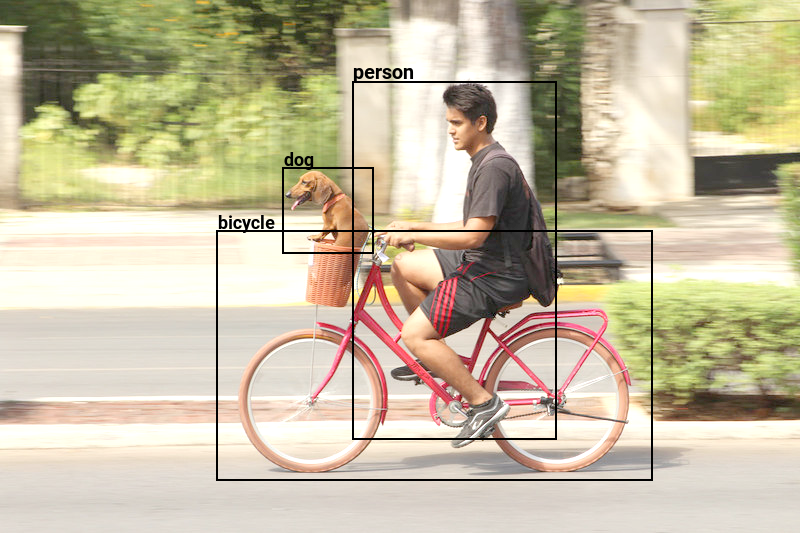
\includegraphics[width=\textwidth]{dogbike_annotated}
\centering
\caption{Visualization of the labels and bounding boxes emitted by YOLO when given an image depicting a cyclist with a dog.}
\end{figure}

YOLO is written in C, using the Darknet neural network library \citep{darknet13}.
It can be used in Python with the TensorFlow machine learning library and the Darkflow library which translates a Darknet model to TensorFlow.

When invoked from Python, the return value is a collection of dict objects, each containing a label, coordinates and a confidence score.
This data is cast into a TTR record as described in \autoref{ssec:python}.

\begin{lstlisting}[label=lst:yolo_out, caption=Example output of YOLO invocation]
[
	{
		'topleft': {'x': 354, 'y': 86},
		'bottomright': {'x': 551, 'y': 437},
		'label': 'person',
		'confidence': 0.80116189
	},
	{
		'topleft': {'x': 224, 'y': 234},
		'bottomright': {'x': 646, 'y': 476},
		'label': 'bicycle',
		'confidence': 0.85828924
	},
	...
]
\end{lstlisting}



\subsection{Objects}

The perception of objects is largely based on \cite{lspc}.
There, the input space is a 3D point space rather than 2D images.
This difference necessitates other types for the perceptual input and the locations of perceived objects.

[propositions as types, true if there is an object of the type, situation semantics? \cite{BarwiseSituationsAttitudes1981}]
A record of a situation type then serves as a witness for the situation.



\subsection{Spatial relations}
% Classification algorithm non-TTR. Simplistic, compare to sophisitcated alternatives.

Spatial relation classification is mostly based on \cite{ttrspat}, but more simplistic.

\cite{ttrspat} includes two important aspects that are not covered here.
First, it assumes a 3D point space as visual input, in contrast to the 2D image considered here.
Spatial relations in 3D crucially involves adapting the reference frame according to the viewpoint, while those are trivially fixed in the 2D case.
Second, it accounts for the functional aspect of spatial relationship, as detailed by \cite{CoventryClassificationExtrageometricInfluences2004}.

Spatial classifiers $\kappa$ take two locations and return a boolean result.
I have implemented them as Python functions.
For the purpose of this thesis, no sophisticated spatial classification has been considered.
Instead, a naive comparison between centers of bounding boxes was implemented.
This was done for the four relations "left", "right", "above" and "below".



\subsection{Language}
% Why connect language? Is it VQA? Parsing. Classification before or after question.

[highlight how TTR makes it easy to answer a yes/no question]

A dog is to the left of a car
\begin{equation}\left[\begin{array}{rcl}
\text{x} &:& Ind\\
\text{y} &:& Ind\\
\text{c}_\text{dog} &:& \text{dog}(x)\\
\text{c}_\text{car} &:& \text{car}(y)\\
\text{c}_\text{left} &:& \text{left}(x, y)\\
\end{array}\right]\end{equation}


Essentially, we would like to check if the situation observed is a subtype of the situation described by the text/question, whether $Q \sqsupseteq A$. A new problem here is that field labels do not match, even if the field values (the types) match. We thus need to consider all (?) relabelings of $Q$:

A record type $T_1$ is a \textbf{relabel-subtype} of $T_2$, or $T_1 \sqsubseteq_{rlb} T_2$,  iff there is a relabeling of $T_1$, $T_{1_{rlb}}$ where $T_{1_{rlb}} \sqsubseteq T_2$.

(Or: iff $T_1$ is $\Sigma$-equivalent to a subtype of $T_2$?)

Could we forget field labels and just look at the two sets of field values? Not really, because we have dependent types, so $\text{dog}(x_1) ≠ \text{dog}(x_2)$. We need to carry out each candidate \textit{relabeling} and check subtypeness. In practice, and in this case, relabeling the basic-type ($Ind$) fields is enough, because those are the only ones whose labels appear in dependent fields. For each basic-field relabeling, we can then kind of forget labels and just find subtypeness of field values.

[classification before/after question]

Parsing natural language to TTR has been addressed in \cite{CooperRecordsRecordTypes2005}, \cite{RobinCooperAustiniantruthattitudes2005}, \cite{CooperTypetheorysemantics2012}, \cite{CooperTypetheorylanguage2016}.
These accounts cover basic grammar, and are likely enough for the kind of utterances considered here.
It would have been interesting to see also those implemented here.
However, to save time I went for a simpler approach using NLTK's feature structure CFG.
With a custom Python function, the FOPC output is transformed to a TTR record type.



\subsection{Evaluation}

The system is tested on a few sentences for a few images.
...
